\documentclass[preprint]{aastex}
\usepackage{newtxtext, newtxmath}

\usepackage{graphicx}
\graphicspath{
  {../},
}


\usepackage{geometry}
\geometry{margin=1in}
\setkeys{Gin}{width=0.6\linewidth, keepaspectratio}  

\usepackage{natbib}
\usepackage{microtype}
\bibliographystyle{apj}


\newcommand\Pixel{\ensuremath{\Omega_{\mathrm{pix}}}}
\newcommand\Area{\ensuremath{A_{\mathrm{HST}}}}
\newcommand\T[2]{\ensuremath{T_{#1}^{#2}}}
\newcommand\Tlam[1]{\T{\lambda}{#1}}
\newcommand\Tmax[1]{\T{\mathrm{m}}{#1}}
\newcommand\Mean[1]{\ensuremath{\bigl\langle \lambda I_\lambda \bigr\rangle_{#1}}}
\newcommand\MeanC[1]{\ensuremath{\bigl\langle \lambda
    I_\lambda^{\mathrm{cont}} \bigr\rangle_{#1}}}
\newcommand\Color[2]{\ensuremath{k_{#1, #2}}}
\newcommand\COLOR[2]{\ensuremath{\widetilde{k}_{#1, #2}}}
\newcommand\Weff[2]{\ensuremath{\widetilde{W}_{#1, #2}}}
\newcommand\U[1]{\ensuremath{\mathrm{#1}}}
\newcommand\E[1]{\ensuremath{\times 10^{#1}}}
\newcommand\Elam{\ensuremath{\varepsilon_\lambda}}
\newcommand\Constant{\ensuremath{C_{\mathrm{WFC3}}}}


% \newcommand\Narrow{\mathrm{L}}
% \newcommand\Wide{\mathrm{C}}
% \newcommand\Narrow{\mathrm{a}}
% \newcommand\Wide{\mathrm{b}}
\newcommand\Narrow{\mathrm{N}}
\newcommand\Wide{\mathrm{W}}
\newcommand\Contam{\ensuremath{{i'}}} %extra braces are on purpose

\begin{document}
\title{Temperature and density fluctuations in the inner Orion Nebula}
\author{W. J. Henney, C. R. O'Dell, G. J. Ferland, M. Peimbert}
\section{Analysis}
\label{sec:fluct}



\subsection{Deriving diagnostic line ratios from WFC3 filter images}
\label{sec:filters}
\begin{figure}
  \centering
  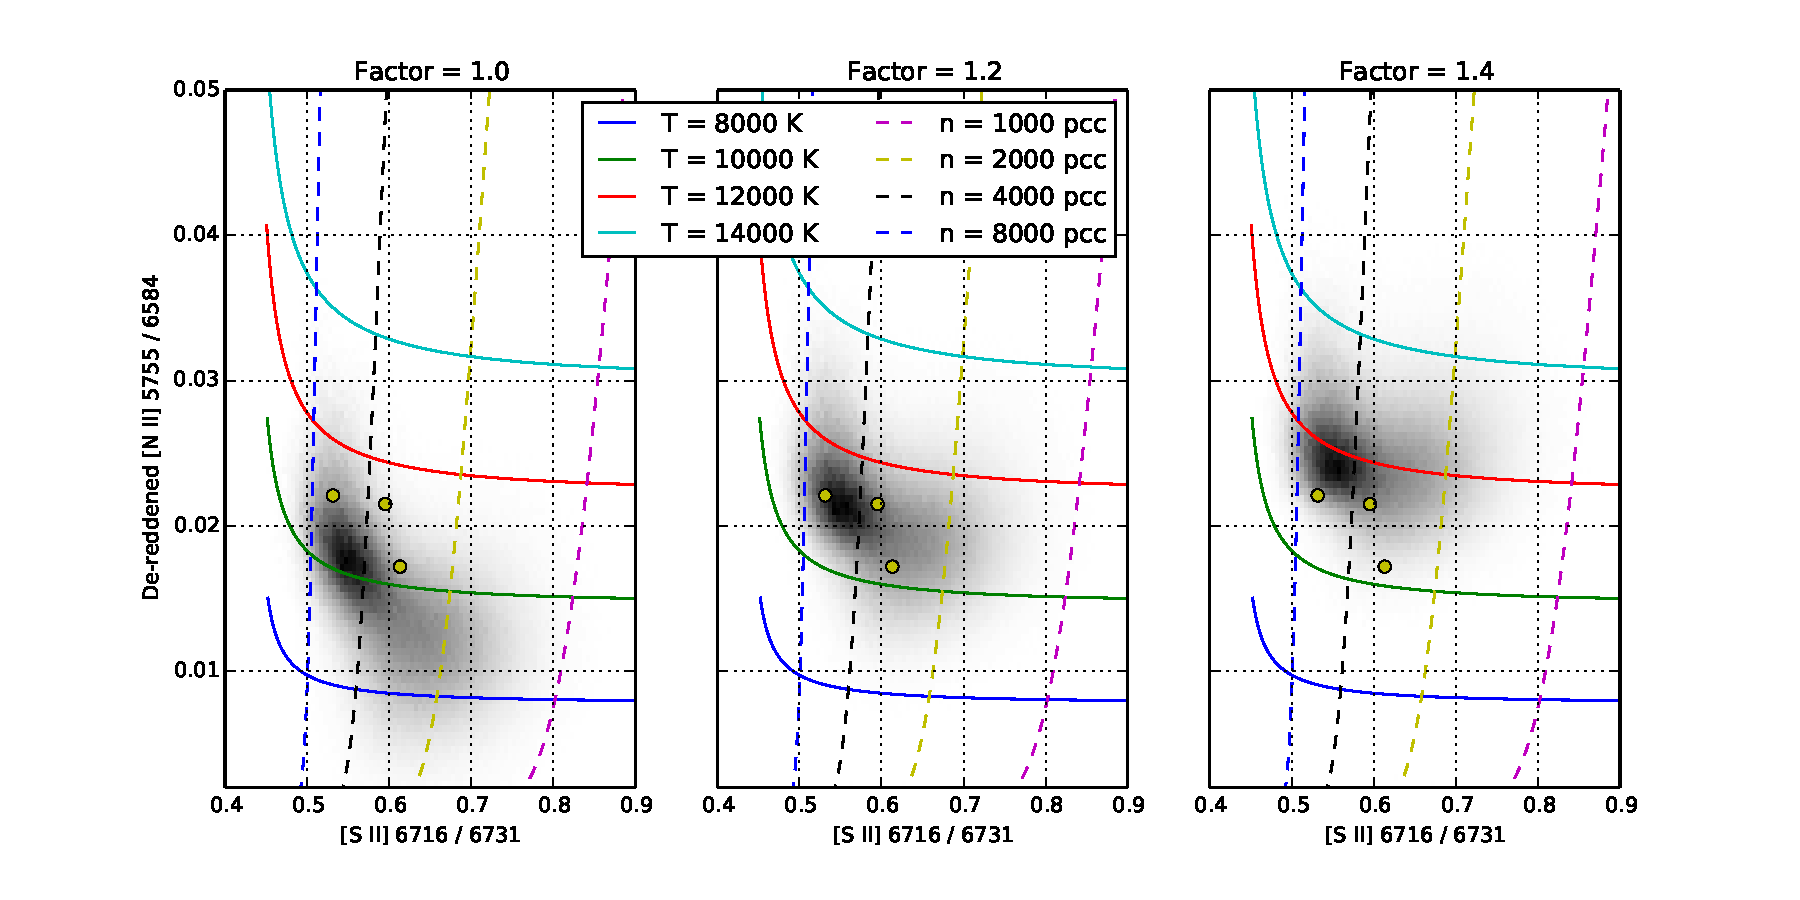
\includegraphics[width=\linewidth]{bivar_rsii_rnii_multifactor}
  \caption{Distribution of line ratios}
  \label{fig:line-ratios}
\end{figure}

\textit{Note: this is similar to what I wrote in the the calibration
  draft, but specifically tailored to line ratios rather than
  equivalent widths.  We may in the end want to move some of it back
  to the other paper.}

The WFC3 camera is equipped with filters that effectively target
important nebular diagnostic lines.  Each filter, with label \(j\), is
characterized by an effective transmission profile, or throughput,
\Tlam{j}, which gives the wavelength-dependent conversion factor
between the number of photons arriving at the \textit{HST} entrance
aperture (nominal radius: \(120\ \U{cm}\)) and the number of electrons
registered by the CCD, accounting for occultation by the secondary
mirror, all other optical and quantum efficiencies, and the amplifier
gain.  The peak value of the filter transmission profile is denoted
\Tmax{j}, with typical values of 0.2--0.3, and the ``rectangular
width'' of the profile is defined as
\begin{equation}
  \label{eq:width}
  W_j = (\Tmax{j})^{-1} \int_0^\infty \!\!\Tlam{j}\, d\lambda 
  \quad\quad [W_j] = \U{\AA}.
\end{equation}


Extensive and continuing on-orbit calibration of the filters has been
carried out \citep{Kalirai:2009a, Kalirai:2010a, Sabbi:2013b} using
white dwarf standard stars.  However, since these are flat featureless
continuum sources, the calibration is only sensitive to the integrated
filter throughput, given by the product \(W_j \Tmax{j}\).  A general
increase in the integrated throughput of 10--20\% with respect to
pre-launch measurements was found for all filters, which was fitted by
a low-order polynomial as a function of frequency.  Only the
broad-band and medium-band filters were used in determining the fit,
but the scatter of the narrow-band filters\footnote{Note, however,
  that the quad filters were not included in these studies.} around
the resulting curve is only a few percent (see Fig.~6 of
\citealp{Kalirai:2009a}).

Emission lines from photoionized regions are intrinsically much
narrower than even the narrowest WFC3 filters, so the transmission of
such a line, with label \(i\), is independent of \(W_j\) and depends
instead solely on the throughput at the line wavelength: \(\T{i}{j}
\equiv \Tlam{j}(\lambda\!=\!\lambda_i)\).  The detailed shape of the
throughput curves was measured pre-launch \citep{Brown:2006a}, but
direct on-orbit confirmation of these curves is impossible.  However,
by comparing WFC3 images with ground-based spectrophotometry of
emission line nebulae, it is possible to test the filter calibrations
for the case where emission lines are the dominant component of the
spectrum in the filter bandpass.  Just such a calibration is described
in detail in a companion paper \citep{Henney:Calibration}, using
multiple spectrophotometric datasets of the Orion Nebula (M42) and the
evolved nearby planetary nebula NGC~6720 (the Ring Nebula), and
building on an earlier study in \citet{ODell:2013b}.  The conclusion
of this study is that the nominal filter parameters (that is, the
pre-launch measurements of the shape of the throughput curve \Tlam{j},
combined with the on-orbit re-calibration of \(W_j \Tmax{j}\)), are
consistent to within \(\pm 5\%\) with the emission line
spectrophotometry for all but a handful of filters.  The largest
discrepancy is found for the F469N filter, which is found to have a
sensitivity to the \ion{He}{2} \Wav{4696} line that is 35\% higher than the
nominal value.  However, that line is absent in M42, due to the
relatively low effective temperature of the ionizing star, and the
filter is instead dominated by continuum and weak [\ion{Fe}{3}]
lines.  In such circumstance the nominal F469N parameters are found to
be accurate.  

Smaller, but still significant, discrepancies are found for the F658N
and FQ575N filters, which target the \nii{} lines \Wav{6583} and
\Wav{5755}, respectively. \textit{Discuss inconsistency between Ring
  and Orion calibration.  Ring has 5755 increased by 10\%.  Orion has
  6583 decreased by 10\%.  But effects on ratio are similar.}

We model the specific intensity, \Ilam (in \U{erg\ s^{-1}\ cm^{-2}\
  sr^{-1}\ \AA^{-1}}), of a spatially resolved astrophysical source as
the sum of several narrow emission lines \(i\), each with central
wavelength \(\lambda_i\) and wavelength-integrated intensity \(I_i\),
plus a slowly varying continuum \Icont:
\begin{equation}
  \label{eq:line-plus-cont}
  \Ilam = \Icont + \sum_{i=1, n} I_i\, \delta(\lambda - \lambda_i)  ,
\end{equation}
where \(\delta\) denotes the Dirac delta function.   It is convenient
to define an average continuum intensity over the passband of filter \(j\): 
\begin{equation}
  \label{eq:average}
  \MeanC{j} = \int_0^\infty \!\!\lambda \Icont  \Tlam{j} \, d\lambda \,
  \Bigg/\! \int_0^\infty \!\!\Tlam{j} \, d\lambda .
\end{equation}
The count rate (in \U{e^-/s}) in a single pixel of a pipeline-reduced
(bias-subtracted, flat-fielded, drizzled) WFC3 image should then be
\begin{equation}
  \label{eq:R-line-plus-cont}
  R_j 
  = \Constant\,
  \left(
    \MeanC{j} \, \Tmax{j} W_j 
    + \sum_{i=1,n} \lambda_i I_i \T{i}{j}
  \right)
\end{equation}
where \(\Constant = 10^{-8} \Area\, \Pixel / (h c) = 0.0840241\
\U{counts\ cm^2\ sr\ erg^{-1}\ \AA^{-1}\ pixel^{-1}}\) is a constant
for the camera, depending on the telescope aperture area, \(\Area =
\pi (120\ \U{cm})^2 = 45,239\ \U{cm^2}\), and the solid-angle
subtended\footnote{Although geometric distorsions by the telescope
  optics mean that the true pixel area varies across the field of
  view, this is corrected for during the ``drizzle'' stage of the
  pipeline reduction process, which yields images interpolated onto a
  regular pixel grid.  If non-drizzled images are used, then a further
  correction for the pixel area map must be applied to equation~(\ref{eq:R-line-plus-cont}).} by each pixel
\(\Pixel = (0.03962'')^2 = 3.6895\E{-14}\ \U{sr}\).




\(R_{\scriptscriptstyle \mathrm{III}}\)

\subsection{\boldmath Deriving \(\Te, \Ne\) from line ratios}
\label{sec:derive}

\begin{figure}
  \centering
  \begin{tabular}{ll}
    (\textit{a}) & (\textit{b}) \\
    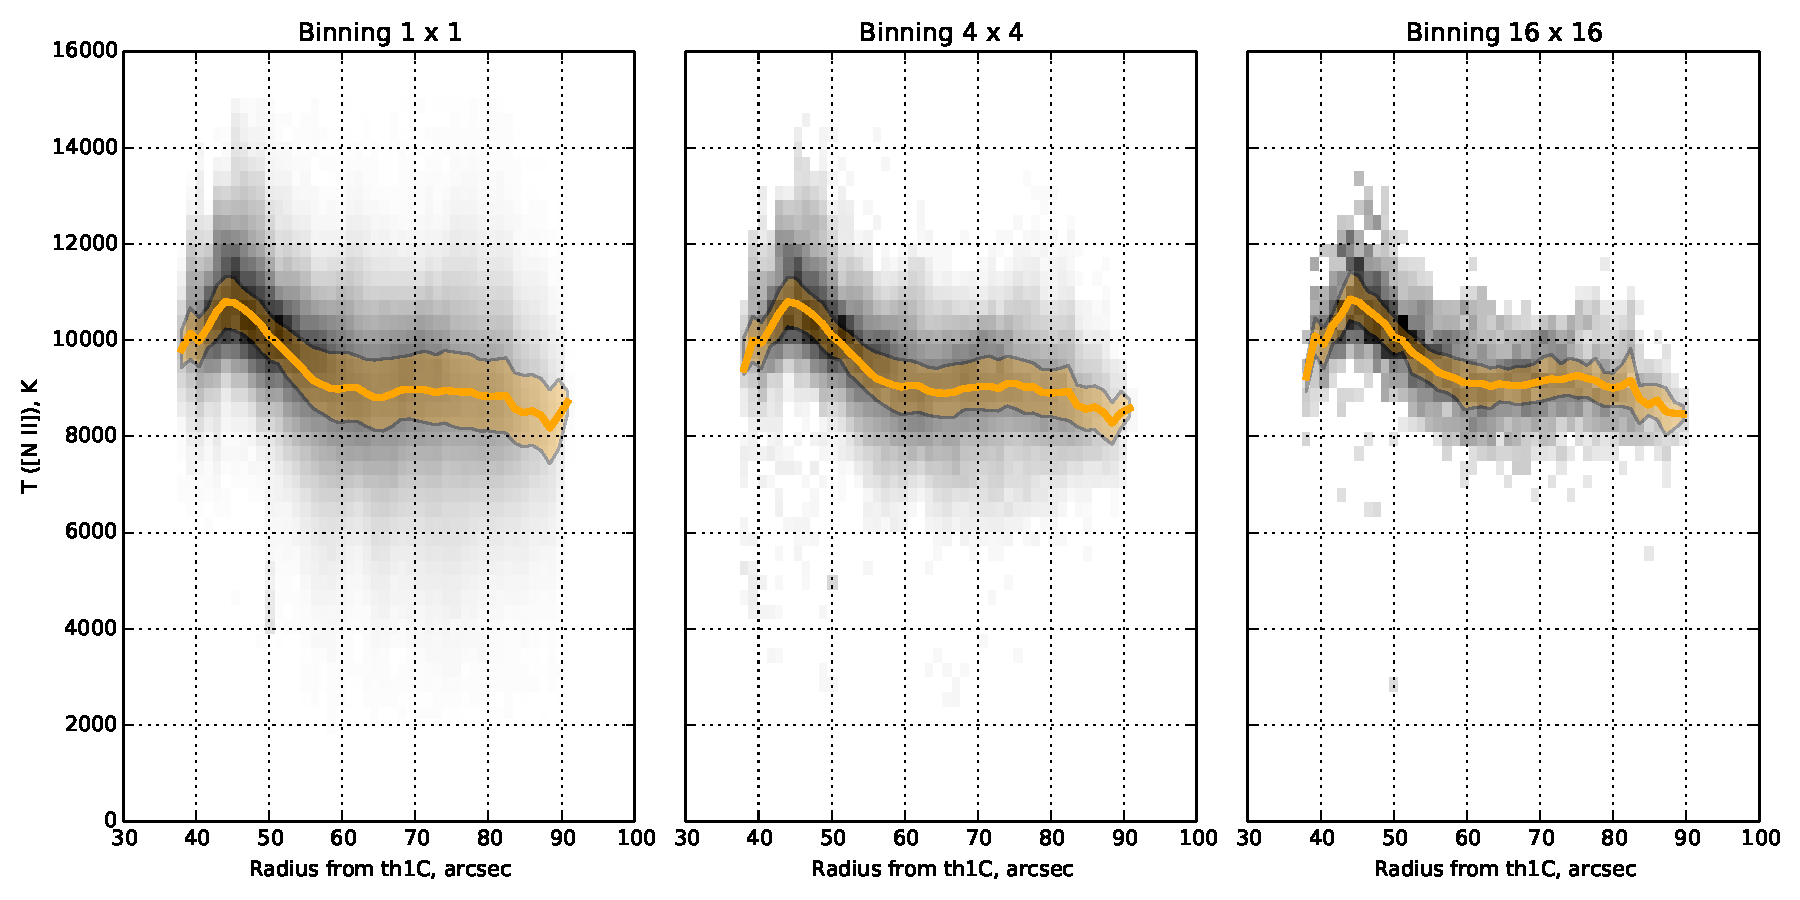
\includegraphics[height=0.35\textheight]{Tnii-vs-radius-binning} &
    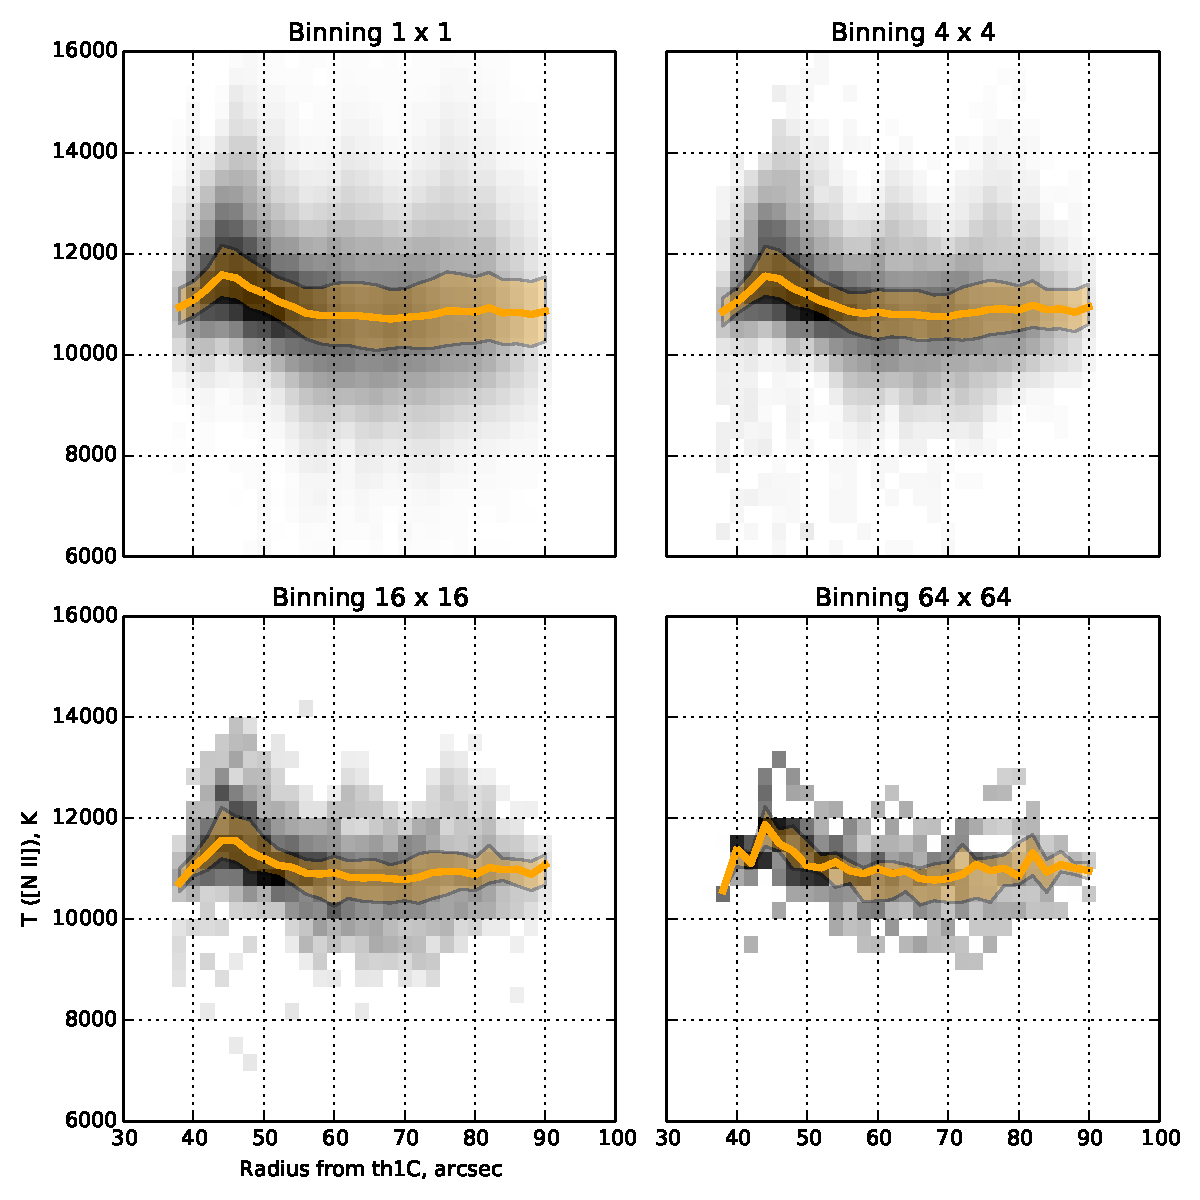
\includegraphics[height=0.25\textheight]{sigma-Tnii-vs-radius-binning}
  \end{tabular}
  \caption{(\textit{a})~Temperature distribution as a function of
    radius for different binnings.  (\textit{b})~Standard deviation of
    temperatures as a function of radius for different binnings. 
  }
  \label{fig:tnii-vs-rad}
\end{figure}


\subsection{\boldmath Analysis of fluctuations in \(\Te, \Ne\)}
\label{sec:fluct}


\begin{figure}
  \centering

  \begin{tabular}{ll}
    (\textit{a}) & (\textit{b}) \\
    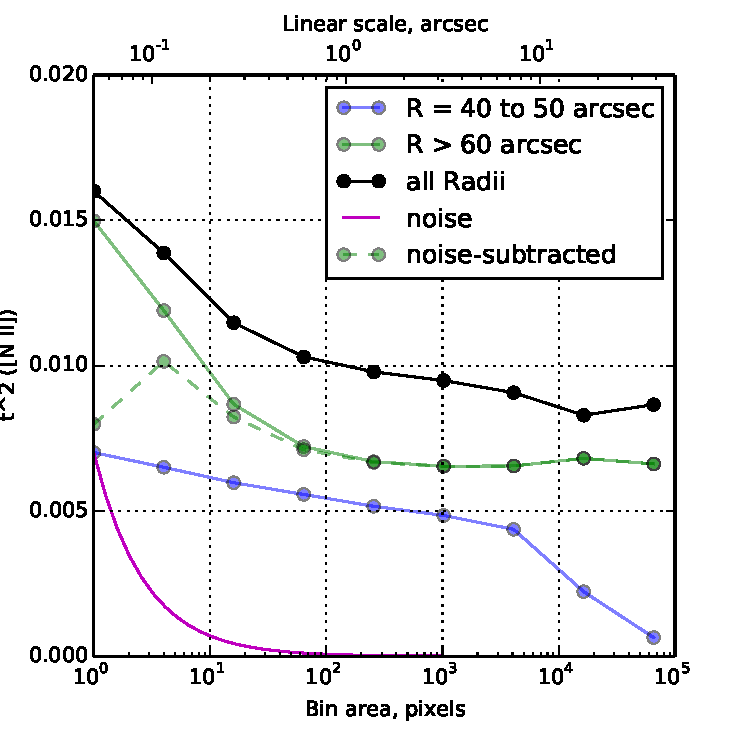
\includegraphics[width=0.45\linewidth]{Tsq-nii-vs-binning-normal} &
    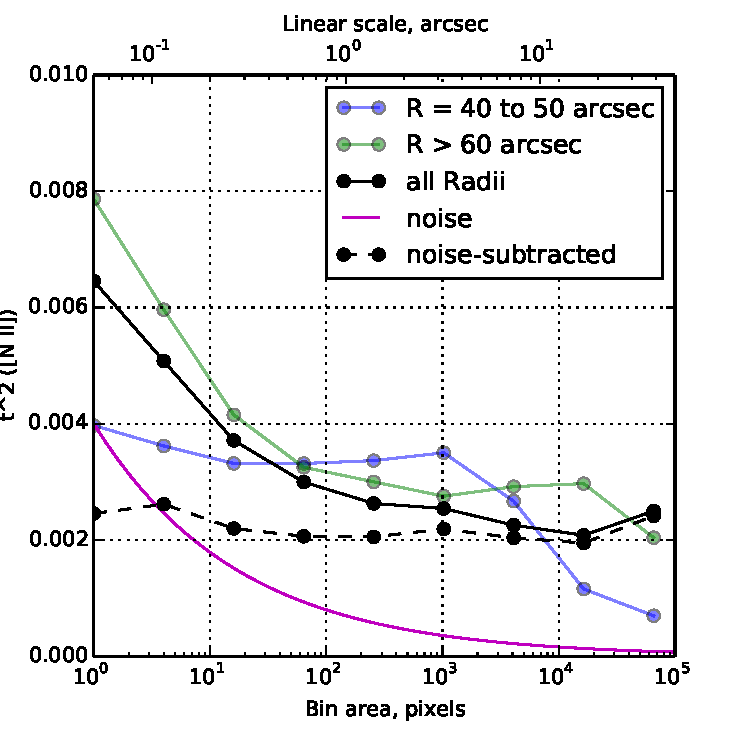
\includegraphics[width=0.45\linewidth]{Tsq-nii-vs-binning-robust}
  \end{tabular}
  \caption{Scale-dependence of temperature fluctuations: \(t^2\) as a
    function of binning. (\textit{a})~Variance of \(\Te/\bar{\Te}\)
    for the entire image (black line) and two subsamples: an annulus
    centered on the high-temperature region (blue line) and the more
    distant, fainter regions (green line).  The magenta line is an
    estimate of the noise contribution to the full sample, and the
    dashed black line is the result of subtracting the noise from the
    observed values.  (\textit{b})~Same as \textit{a} but using a
    ``robust'' estimator of the variance, based on the interquartile range.}
  \label{fig:tsq-nii-vs-binning}
\end{figure}


\begin{figure}
  \centering
  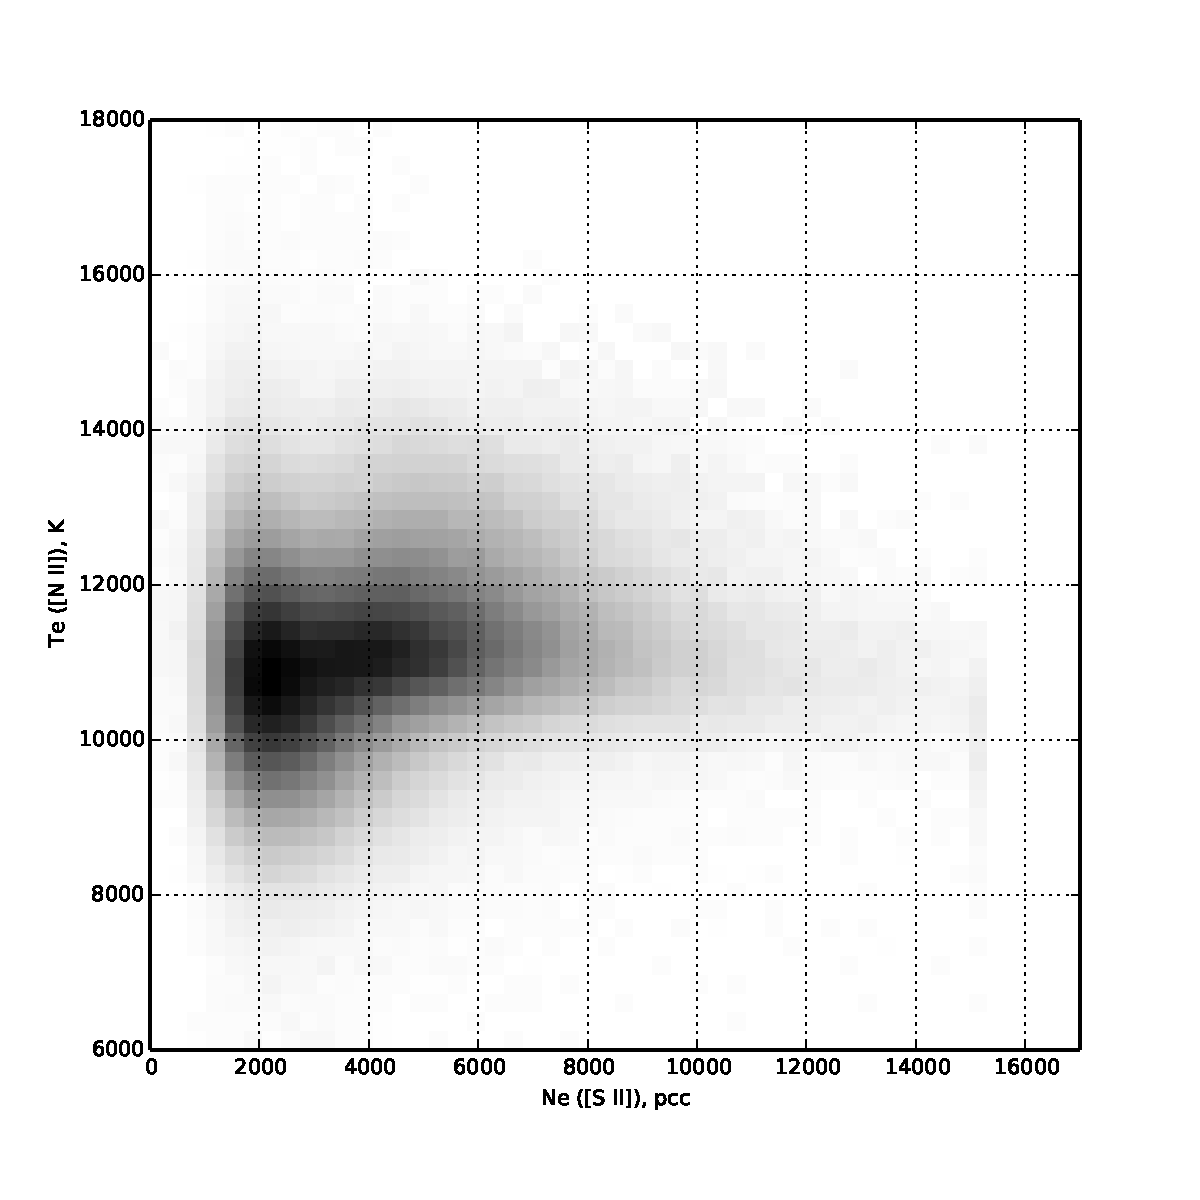
\includegraphics[width=0.8\linewidth]{Te-versus-Ne}
  \caption{Joint distribution of temperature and electron density for
    low ionization regions.}
  \label{fig:Te-Ne}
\end{figure}

\begin{figure}
  \centering
  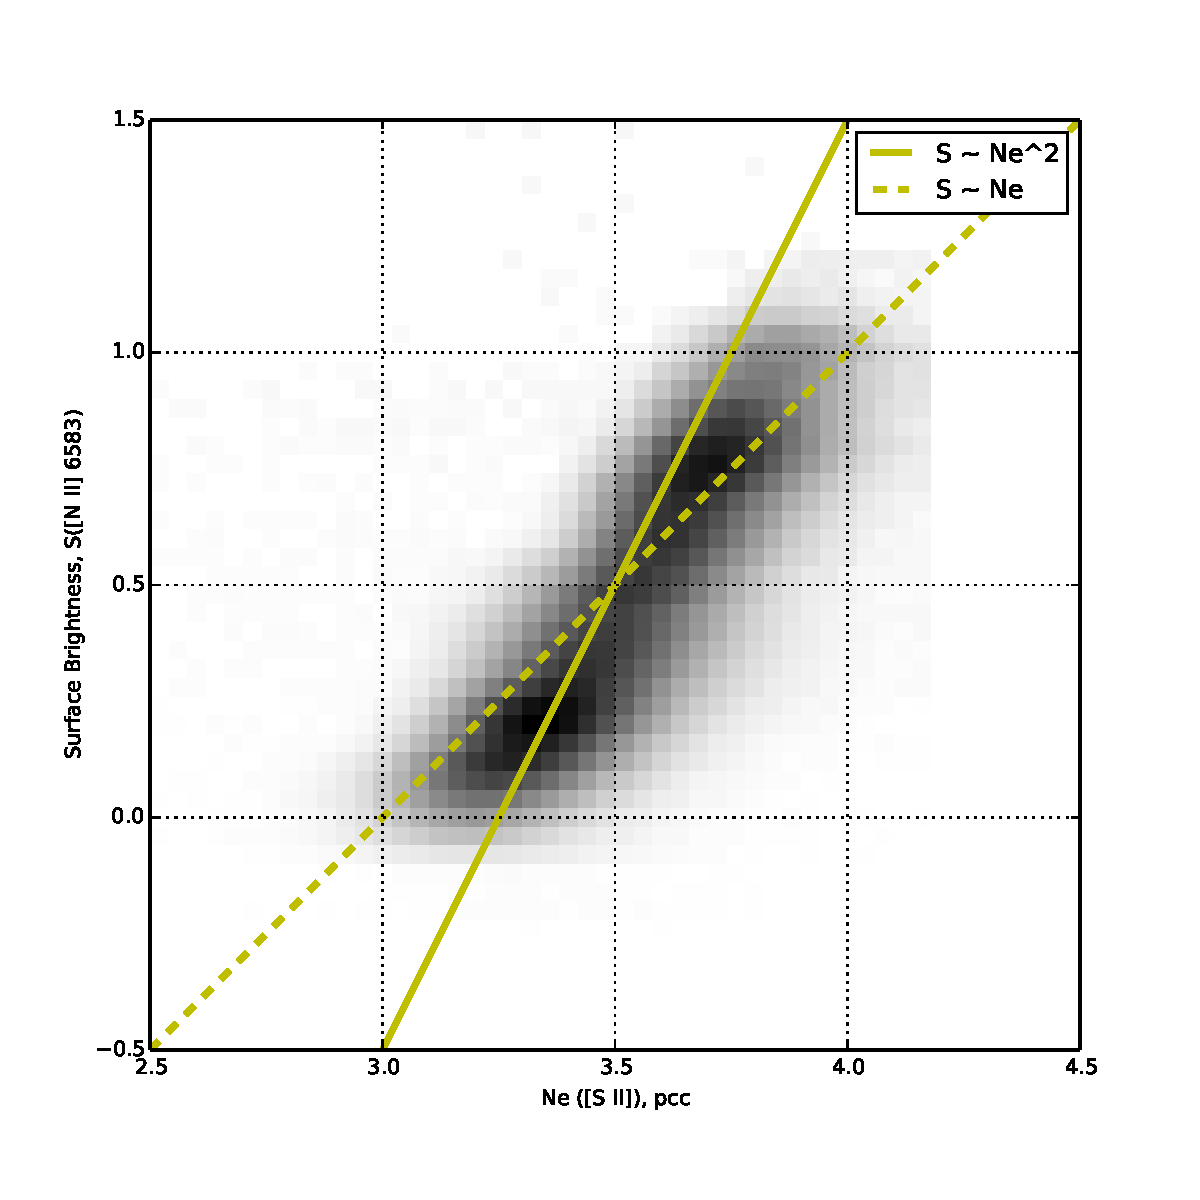
\includegraphics[width=0.8\linewidth]{snii-versus-ne}
  \caption{Correlation between \sii{} density and \nii{} surface brightness.}
  \label{fig:Snii-ne}
\end{figure}


\bibliography{BibdeskLibrary-slavoj}


\end{document}
